\chapter{Problemforståelse}
Denne fasen eksisterer for å passe på at en har forstått problemet i dypere detalj. Verktøyene som er relevante å bruke skal gi en bedre forståelse av blant annet omfanget og de ulike aspektene ved et problem. Jo bedre tilgang en har på logger og dokumentasjon, jo bedre vil denne fasen kunne utføres. Siden vi har liten erfaring med bruk av verktøy vil vi prøve ut to i denne analysen. Kritiske hendelser for å undersøke hva som blir lastet ned, og flytdiagram for å kartlegge hendelsesforløpet til en som laster ned.

\section{Flytdiagram}
Et flytdiagram er et diagram som viser en flyt av aktiviteter i en prosess eller handling. Flytdiagrammer kan bli brukt til å kartlegge en prosess for å muligens illustrere hvor problemet ligger, eller for å skape en grunnleggende forståelse av prosessen som har innflytelse på problemet. 

\subsection{Ønsket utbytte}
Her prøver vi å kartlegge hendelsesforløpet, og hvordan bruksmønsteret til en bruker av nettet til NTNU kan se ut, da med fokus på fildeling. Vi håper at dette kan gi oss en mer helhetlig forståelse av hva som kan være årsaken til fildeling, og kanskje vi kan bruke dette til å komme opp med tiltak senere i prosessen.
\subsection{Gjennomføring}
Vi fulgte metoden for å lage et flytdiagram, fra boken om rotårsaksanalyse \cite{RCA}.
\begin{enumerate}
    \item Vi samlet alle på gruppen for å diskutere prosessen, og hadde med oss post-it lapper
    \item Vi definerte brukerne som studenter ved NTNU og da, antageligvis mest studenter som bor på studenthybler.
    \item Vi definerte hvilke aktiviteter som må bli gjort/være tilstede for at skolen skal få et notis.
    \item Så flyttet vi rundt på lappene til de kom i en naturlig rekkefølge.
\end{enumerate}


For å forstå problemet lagde vi et flytdiagram for å få en bedre forståelse av hendelsesforløpet når noen driver med fildeling.

\subsection{Resultater}
Flytdiagrammet som ble laget kan sees under. Først kobles en bruker seg til skolenettet, enten gjennom VPN eller direkte fra campus eller studenthybler. Deretter velger brukeren enten å bruke nettet vanlig eller starter å laste ned filer, hvis brukereren bruker det vanlig bryr vi oss ikke om disse. Når vedkommende som har bestemt seg for å laste ned skal laste ned har han muligheten til å gjøre dette gjennom en privat nedlastingsside. Vi gjør den antagelsen her at private tjenester ikke er med i statistikken fra skolen og at det ikke kommer noen opphavsrettsnotiser fra brukere som bruker private tjenester. Med private tjenester mener vi lukkede nettsamfunn som bare er til for å distribuere opphavsrettsbeskyttet materiale gratis. Det neste som kan skje med de som bruker offentlige tjenester er at de torrentene de laster ned blir sporet, og da får domeneeier et notis om ulovlig nedlasting.
\begin{figure}[H]
    \centering
    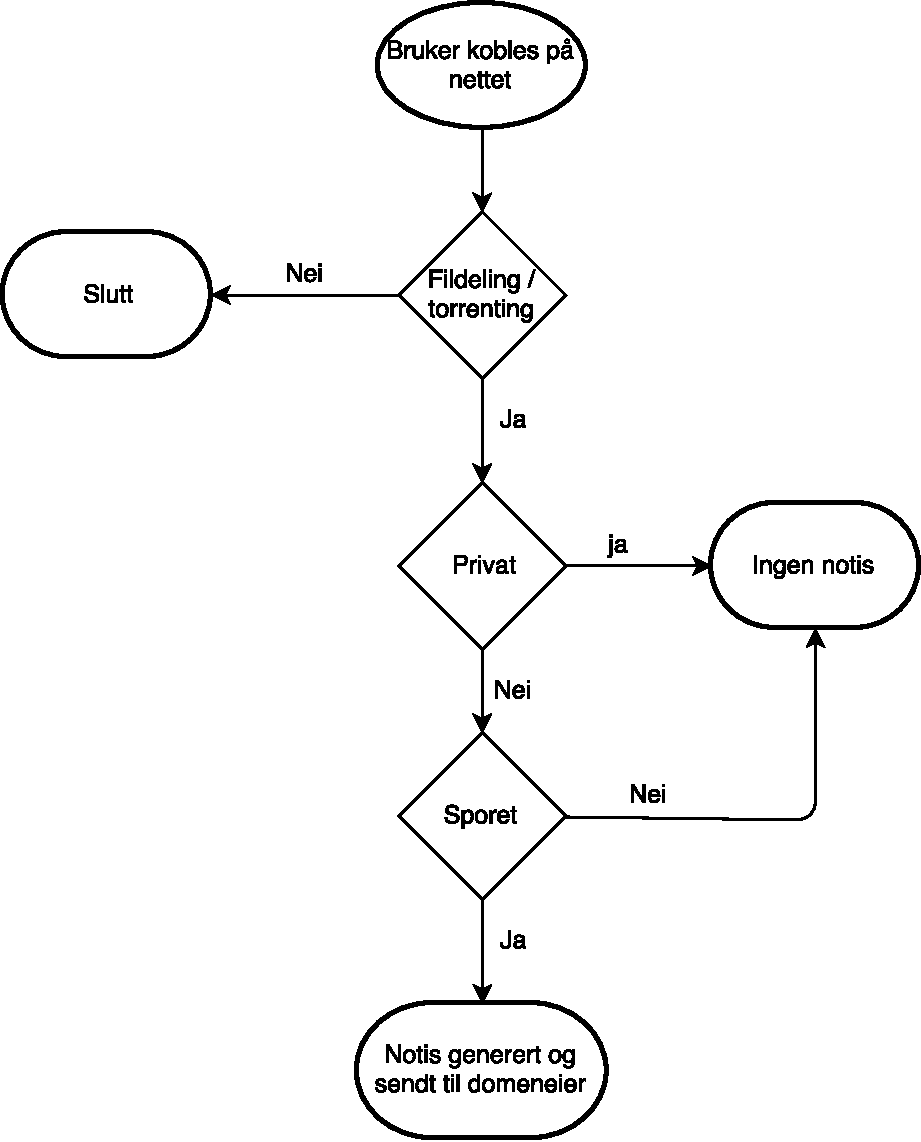
\includegraphics[scale=0.5]{case_1/bilder/Flowchart.pdf}
    \label{fig:Flytdiagram}
    \caption[Flytdiagram for fildeling]{Flytdiagram for fildeling}
\end{figure}

\subsection{Konklusjon av verktøyet}
Vi følte verktøyet fungerte godt for å få et overblikk på hvordan situasjonen med torrenting fungerte. Eneste negative med verktøyet er at det krever ganske god kjennskap til mulige hendelsesforløp, noe som kan være negativt om man ikke kjenner godt til problemet fra før. 

\section{Kritiske hendelser}
For å gå dypere i detalj har vi tatt en titt på kritiske hendelser som inngår i problemstillingen. Vi har valgt å dele opp problemet i mindre stykker for å spørre studenter som bor i SiT-bolig om hva de laster ned hvis de først gjør det. 

\subsection{Ønsket utbytte}
Ved bruk av dette verktøyet ønsker vi å få en dypere forståelse av hva studentene laster ned slik at vi kan se om det er noen kategorier som er mest fremtredende. Dette kan føre til at vi blir mer effektive i senere arbeid da vi kan fokusere på det som er viktigst.

\subsection{Gjennomføring}
Det første som ble gjort var å definere de mest relevante kategoriene av nedlastningsmateriale. Dette ble basert på egen erfaring med blant annet hyppigheten til de ulike kategoriene. Vi hadde en viss anelse om hvilke som var de store synderne, men ønsket å bekrefte våre mistanker. Følgende kategorier ble fremhevet: 
\begin{itemize}
    \item Filmer og serier
    \item Skolebøker
    \item Programvare til skolebruk
    \item Programvare og bøker utenom skolebruk
    \item Spill
    \item Musikk
    \item Annet
\end{itemize}

Deretter var det klart for utspørring. Dette var i stor grad uformelle ``intervjuer'' med få spørsmål. Det viktigste vi trengte å vite var om personen bodde i SiT-bolig, siden det er bare beboere derfra som er relevante i vår problemstilling, og fra hvilke kategorier de laster ned fra. Resultatene ble fortløpende ført inn i statistikken. De fleste som ble spurt studerte informatikk, men det ble også spurt noen fra andre linjer for å prøve å balansere det ut. Intervjuobjektene var i stor grad bekjente vi visste bodde i SIT Bolig, og derfor var det en overvekt av IT studenter.

Spørsmål stilt til intervjuobjekter:
\begin{itemize}
    \item Bor du, eller har du bodd i SiT-bolig i løpet av studiet? (Hvis nei, avslutt intervju)
    \item Bruker du, eller har du brukt Torrents til å laste ned opphavsrettsbeskyttet materiale mens du bodde i SiT-bolig? Hvis ja, hvilke av følgende kategorier laster du ned fra? (Viser kategoriene)
\end{itemize}

\noindent Dette er resultatet fra spørringene: \\
\indent Antall spurt: 13 \\
\indent Antall som aldri laster ned: 4
\begin{table} [H]
    \begin{tabular}{ | m{20em} | m{20em} | }
        \hline
            \cellcolor{yellow} Fildelingskategori & \cellcolor{yellow} Frekvens \\
        \hline
            Filmer og serier & 8  \\
        \hline
            Spill & 3 \\
        \hline
            Skolebøker & 2 \\
        \hline
            Musikk & 2 \\
        \hline
            Programvare og bøker utenom skolebruk & 1 \\
        \hline
            Programvare til skolebruk & 0 \\
        \hline
            Annet & 0 \\
        \hline
    \end{tabular}
    \caption{Oversikt over kvantiteten av kritiske hendelser ved torrenting av opphavsrettsbeskyttet materiale}
    \label{kritisk_tabell_1}
\end{table}

Merk: Hver person kan svare at de laster ned fra flere kategorier.

\noindent Vi kan se at det er filmer og serier som er den med størst frekvens i undersøkelsen, noe som bekreftet vår hypotese. Dette funnet vil tilsi at vi kan fokusere mye mer på filmer og serier senere i prosessen siden vi vet dette er en stor del av problemet. 

\subsection{Konklusjon av verktøyet}
Verktøyet bekreftet vår hypotese i at det meste som blir lastet ned på skolens nett er filmer og serier. Dette kan tas til videre betraktning senere i rotårsaksanalysen. Verktøyet fungerte bra og ga oss den informasjonen vi var ute etter. Den fungerer også greit om man ikke har en hypotese om omfang på forhånd slik vi hadde, så lenge en er flinke med idémyldring av mulige kategorier. 